
\section{Implementation}
In the beginning and during the project the group were given ideas and guidelines on which practices that could be applicable to a software development project. Depending on the type and size of a project some practices suit better than others and some practices needs adjustments to gain value for the group. In this section the choices, adjustments and implementation of project practices will be presented.



I följande kapitel redovisas viktiga beslut, förändringar och anpassningar som gjorts 
i projektmetod, projektpraktiker, värderingar, beslut mm som gjorts under studiens genomförande.
(Här kan det vara lämpligt med en indelning i olika ansvarsområden inom projektet?)

\subsection{Project Manager (Caroline)}
Genomförandet av iterationer följer helt och hållet mallen för s k ”sprint” i Scrum [ref] 
och beskrivs enklast med följande aktivitetsdiagram, se  bild
\begin{figure}[htbp]
    \centerline{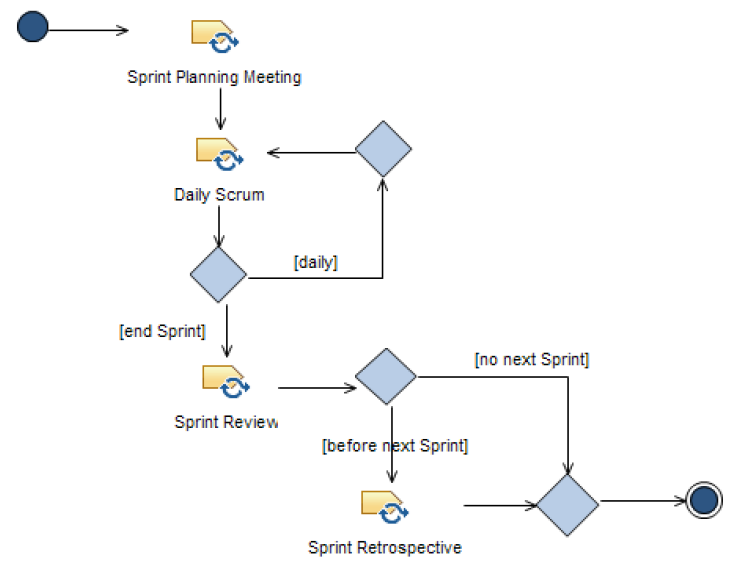
\includegraphics[max height=250px, max width=250px]{Z. images/sprint.png}}
    \caption{Iteration/Sprint}
    \label{fig}
\end{figure}

\subsection{Customer representation (Natasha)}
Lite innehåll.

\subsection{Architecture (Jesper)}


\subsection{Development (Wilhelm)}


\subsection{Testing (Arif)}


\subsection{Sustainability (Gustav)}

